\documentclass{article}
\usepackage{graphicx}
\usepackage{amsmath}

\title{Answers}
\author{Timm Ruland \& Boris Prochnau}

\begin{document}
\maketitle

\begin{itemize}
\section*{Task: 1}	%///////////////////////////////////
	\item What does it do? \\
it prints two not sufficiently seeded "random" variables
	\item The difference between the methods is that rand() returns a random number 
and the other method
  
	\begin{itemize}
		\item rand() returns a random integer between 0 and RANDMAX
		\item gsl\_rng\_mt19937 is a generator that generates random numbers
	\end{itemize}
 In the code the generator is passed to a (Distribution)function that uses this generator 
 to evaluate a random number depending on the Distribution specified in the function.
	\item What happens if you remove the expression (double)?\\
 The division operation $\frac{rand()}{RANDMAX}$ does $\frac{int Small}{int Big}$ and
 should result in a double, but with no cast it will be floored to 0. 
	\item Is there a direct function to generate normally distributed random variables?\\
	double gsl\_ran\_gaussian\_pdf(const gsl\_rng * r, double sigma)
 command
\end{itemize}

\newpage
\section*{Task: 3} %//////////////////////////////////
The Plot should simulate the occurrence density of points of our 1 000 000 samples which are normally distributed. But the picture
shows that all points are over the exact plot of the density function what is nearly impossible with so many samples. Therefore 
we conclude that the plot was made with different parameters.
\begin{figure}[h]
	\centering
		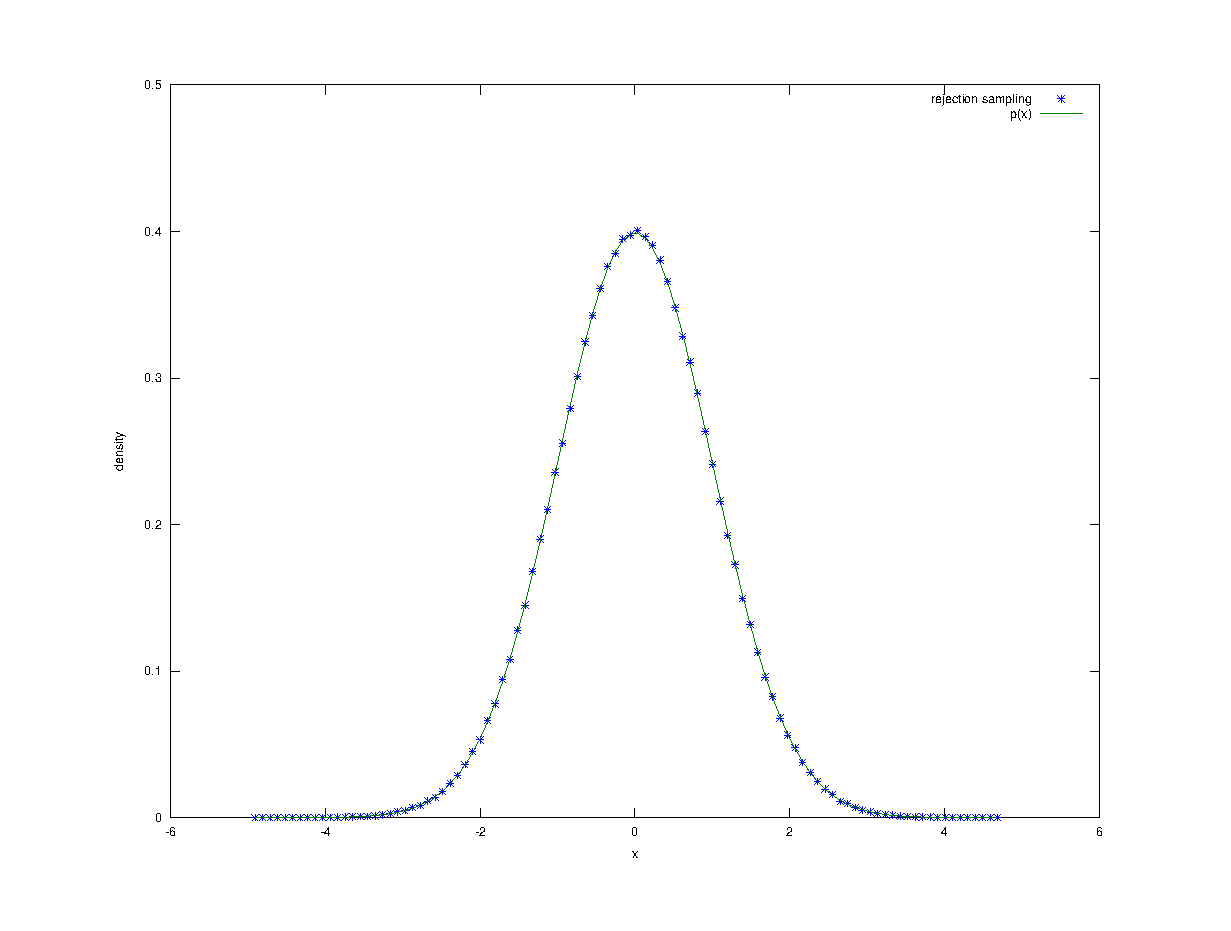
\includegraphics[width=0.70\textwidth]{E:/task3plot.eps}
	\label{fig:task3plot}
\end{figure}

\section*{Task: 4} %//////////////////////////////////
We can sample a uniformlly y in the intervall [0,1] and apply the inverse cdf to sample a normally distributed variable

\newpage
\section*{Task: 5} %//////////////////////////////////
The Algorithm uses a interpolation (see fig. 1) with maximal estimation error: $2\cdot 10^{-9}$ (see fig. 2) where the upper half of the distribution function is divided into 2 sections in which interpolations where made. 
If x is in the lower half of the distribution function, than 1-NomralCDF(-x) will be used to use the symmetric property.
\begin{figure}[htbp]
	\centering
		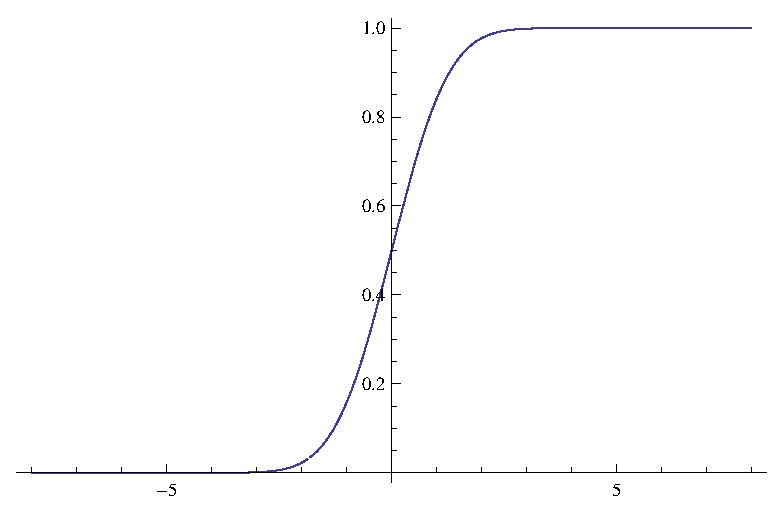
\includegraphics[width=0.60\textwidth]{E:/pics/task5_interpolation_plot.eps}
		\caption{Plot of Approximation}
	\label{fig:task5_interpolation_plot}
\end{figure}
\begin{figure}[htbp]
	\centering
		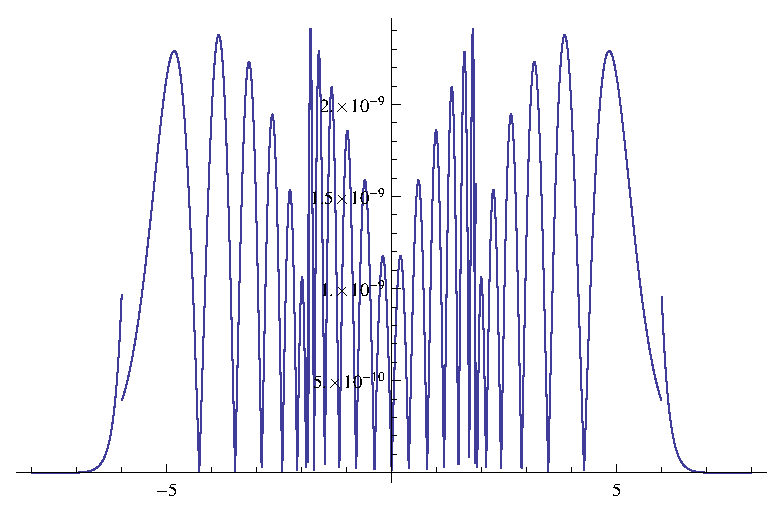
\includegraphics[width=0.60\textwidth]{E:/pics/task5_difference_plot.eps}
	\caption{estimation error}
	\label{fig:task5_difference_plot}
\end{figure}

\newpage
\section*{Task 6}
\begin{figure}[htbp]
	\centering
		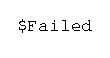
\includegraphics[width=0.50\textwidth]{E:/pics/task6_plot.eps}
	\caption{2D Plot}
	\label{fig:task6_plot}
\end{figure}

\section*{Task 7}
Let $X, Y$ be two independent standard normally distributed random variables. The joint distribution of them is
\[p(x,y) = p(x)p(y) = \frac{1}{\sqrt(2\pi)} e^{-\frac{x^2}{2}} \cdot \frac{1}{\sqrt(2\pi)} e^{-\frac{y^2}{2}} =  \frac{1}{2\pi} e^{-\frac{y^2 + x^2}{2}}\]
We notice that with x,y being two Cartesian coordinates: $x^2 + y^2$ is equal to their radius $r^2$ on a polar circle and we can write:
\[ p(x,y) = \frac{1}{2\pi} e^{-\frac{r^2}{2}}\]
which is the product of two density functions:
\begin{itemize}
	\item $r^2$ ~ Exp($\frac{1}{2}$) so $\lambda = 1/2$.
	\item $\theta$ ~ Unif($0,2\pi$)
\end{itemize}
By using the method of the inverse cdf before, we can now make some interesting computations:
\begin{align*}
y &= 1-\exp(-\lambda x) &|-1&\\
y-1 &= -\exp(-\lambda x) &|\cdot(-1) |\log&\\
log(1-y) &= -\lambda x &|: (-\lambda) &\\
\frac{-log(1-y)}{\lambda} &= x &&
\end{align*}
Therefore we know that the inverse of the exponential distribution function is $F^{-1}(y) = \frac{-\log(1-y)}{\lambda}$. And now we can sample exponentially distributed r.v.'s with the inverse cdf method used before:
\[Exp(\lambda) = \frac{-\log(1-y)}{\lambda} \]
and more important:
\[r\text{~}\sqrt{-\log(Unif(0,1))}\]
with this knowledge we can now sample two uniform distributed r.v.'s $(u_1, u_2)$, one for  $r$ and the other for $\theta$:
\begin{itemize}
	\item $r\text{~}\sqrt{-\log(u_1)}$
	\item $\theta = 2\pi u_2$
\end{itemize}
But those are polar coordinates, so we need to transform them to Cartesian coordinates first:
\begin{itemize}
	\item $x = r \cos (\theta)$
	\item $y = r \sin (\theta)$
\end{itemize}
with these we now got back to a sample from the joint gaussian r.v. what explains why they are normally distributed (with the first equation above).

\section*{Task 8}
The algorithm need only one summation instead of two. The algorithm interates new samples to the total solution of the last step, so it could work better if we constantly give new sampels to the old ones because there is no need to run the hole calculation again. 

\newpage
\section*{Task 9}
We think that the error drops with rate order: $O\left(\frac{1}{\sqrt{N}}\right)$.
\begin{figure}[htbp]
	\centering
		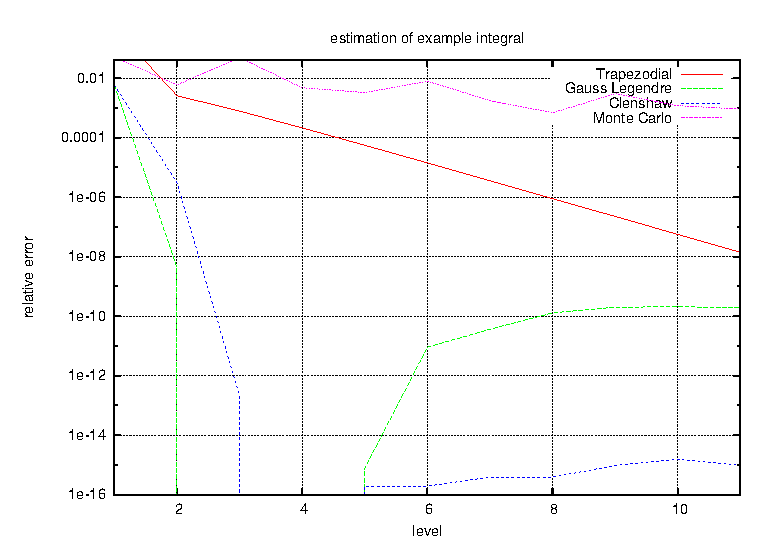
\includegraphics[width=0.70\textwidth]{E:/pics/task9_convergence_plot.eps}
	\caption{estimation error}
	\label{fig:task9_convergence_plot}
\end{figure}

\section*{Task 10}
Do the paths in principal look the same, independent of the time discretization?\\
- We decided that the paths do not look the same because one makes partly rough movements while the other basicly moves with a rate of $\sqrt{t}$.\\
Is the mean change of the price S(t) approximately 10\% /year?\\
- This seems to be possible concerning our Plot listed below. We see that the mean change after 1 and 2 is near the expected 10% raise.
\begin{figure}[htbp]
	\centering
		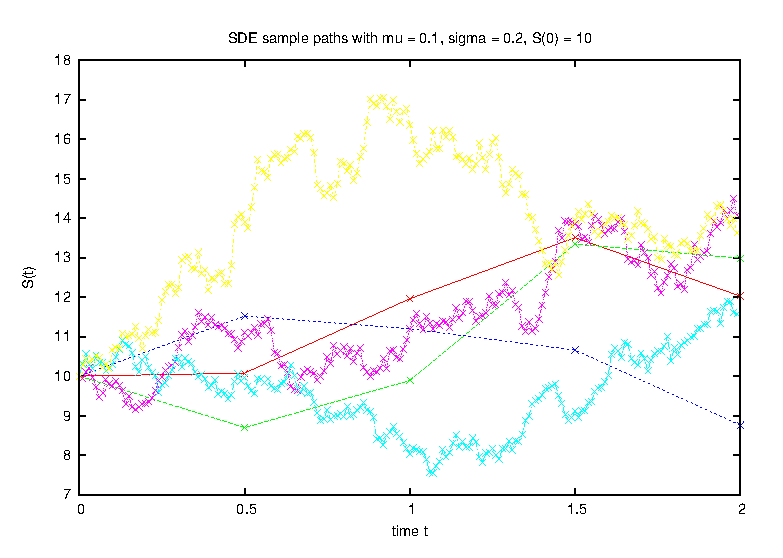
\includegraphics[width=0.70\textwidth]{E:/pics/task10_process_plot.eps}
	\label{fig:task10_process_plot}
\end{figure}
\begin{figure}[htbp]
	\centering
		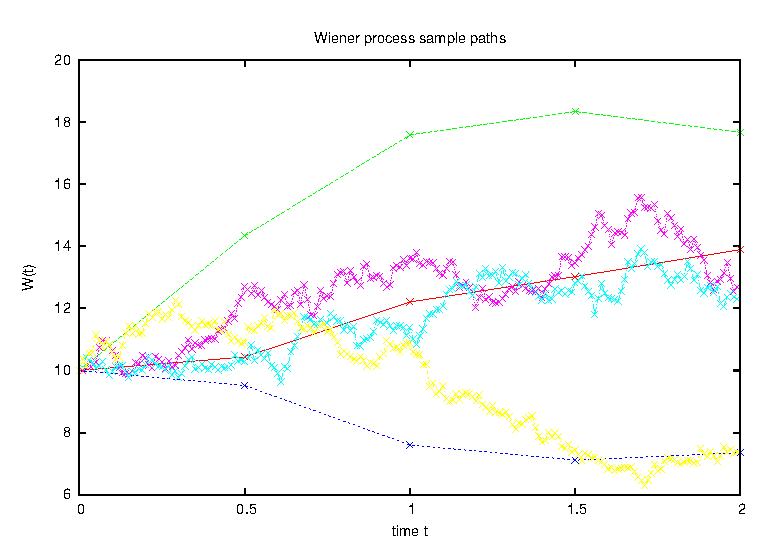
\includegraphics[width=0.70\textwidth]{E:/pics/task10_wiener_plot.eps}
	\label{fig:task10_wiener_plot}
\end{figure}


\end{document}